\section{Depth Map Parameter Tuning}
\label{sec::52_dm}
Within this section, we shortly explore the effects of all tunable parameters on the depth map generation. Therefore, we utilize a simple experimental setup.
%\begin{figure}[h]
%	\centering
%	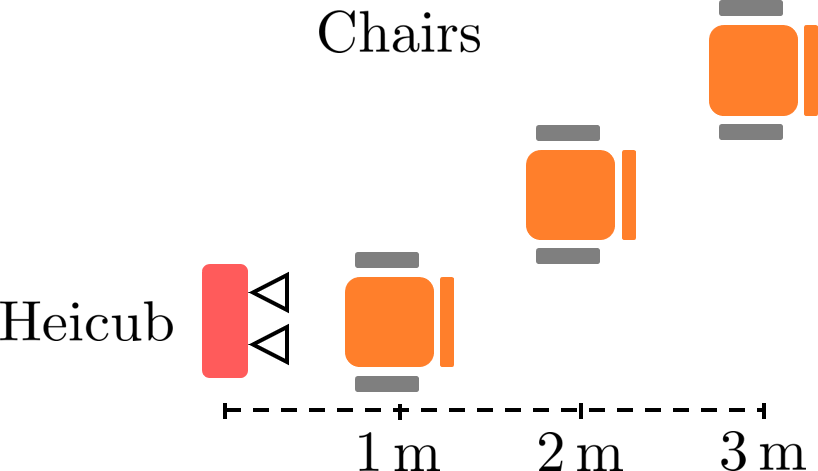
\includegraphics[scale=.4]{chapters/05_experiments/02_depth_map_parameter_tuning/wls_setup.png}
%	\caption{Setup for the parameter tuning of the depth map extraction. Heicub's cameras are indicated by the two triangles, of which you can find the view in figure %\ref{fig::52_wls_rgb}}
%	\label{fig::52_wls_setup}
%\end{figure}
Within the setup, Heicub points its stereo camera towards three chairs that are located at a distance of $1\,\text{m}$ towards each other, and towards the cameras, so to cover close, medium, and far distances. The consecutive chairs are slightly shifted, in order to enable the simultaneous observation of all of them. The rectified view of the environment is shown in figure \ref{fig::52_wls_rgb}.
\begin{figure}[h]
	\centering
	\subcaptionbox{}%
	[.4\linewidth]{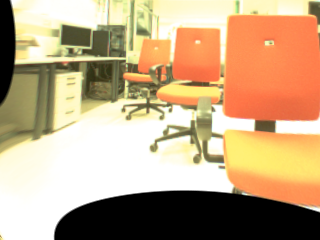
\includegraphics[scale=.3]{chapters/05_experiments/02_depth_map_parameter_tuning/l_rgb.png}}
	\subcaptionbox{}%
	[.4\linewidth]{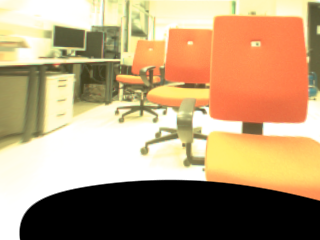
\includegraphics[scale=.3]{chapters/05_experiments/02_depth_map_parameter_tuning/r_rgb.png}}
	\caption{Heicub's perspective of the scene for the setup in figure \ref{fig::52_wls_setup}. (a) shows the left camera's view, while (b) shows the right camera's view.}
	\label{fig::52_wls_rgb}
\end{figure}
The depth map extraction, which utilizes the rectified images, depends on a stereo block matching algorithm that got explained in section \ref{sec::324_ip}. It mainly depends on the window size and the number of disparities for the sum of absolute difference computation. We evaluate the influence of those two parameters in figure \ref{fig::52_disp_sad} in a grid search fashion. It is apparent that the change in the number of disparities has close to no influence onto the depth map quality, while it removes plenty of useful information from the left hand side of images. The same holds true for the window size, except that it removes some noise from the depth maps.
\begin{figure}[h]
	\centering
	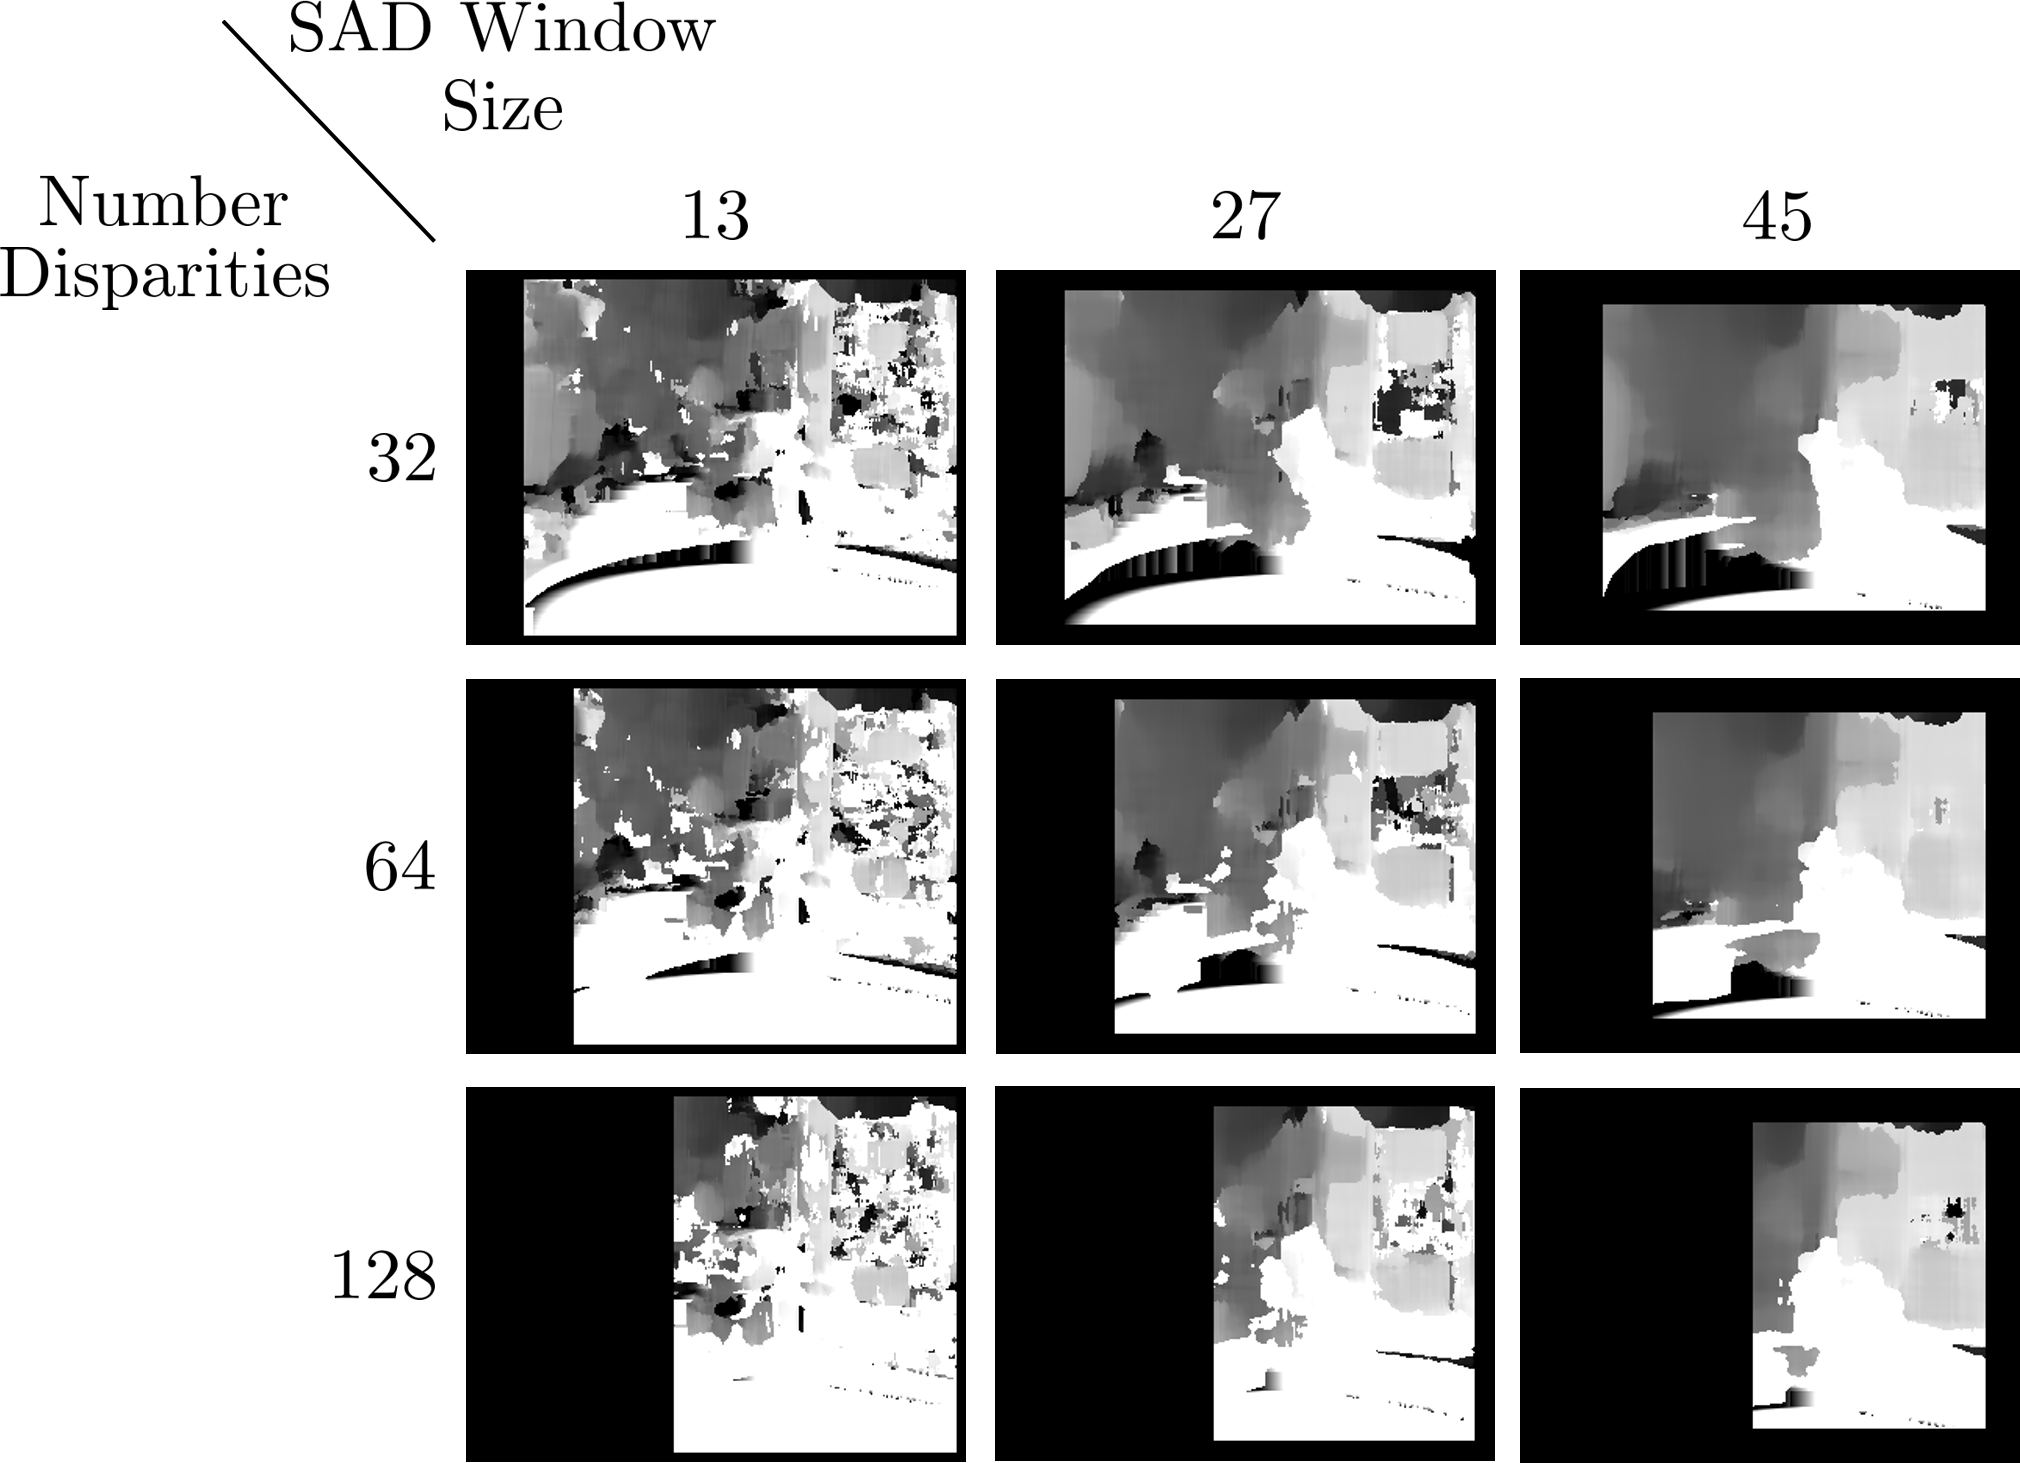
\includegraphics[scale=.25]{chapters/05_experiments/02_depth_map_parameter_tuning/disp_sad.png}
	\caption{Left disparity map for changing SAD window sizes and number of disparities. Please refer to figure \ref{fig::324_left_disparity_map} and equation \ref{eq::324_sad} for the theory.}
	\label{fig::52_disp_sad}
\end{figure}
In combination with the confidence weighted least squares filtering, we can observe that most of the noise is already removed (figure \ref{fig::52_disp_sad_wls}), for which it is more import to keep the information close to the images' borders. We therefore chose to set the number of disparities $D=32$, and the windows size $N=13$ in the following.
\begin{figure}[h]
	\centering
	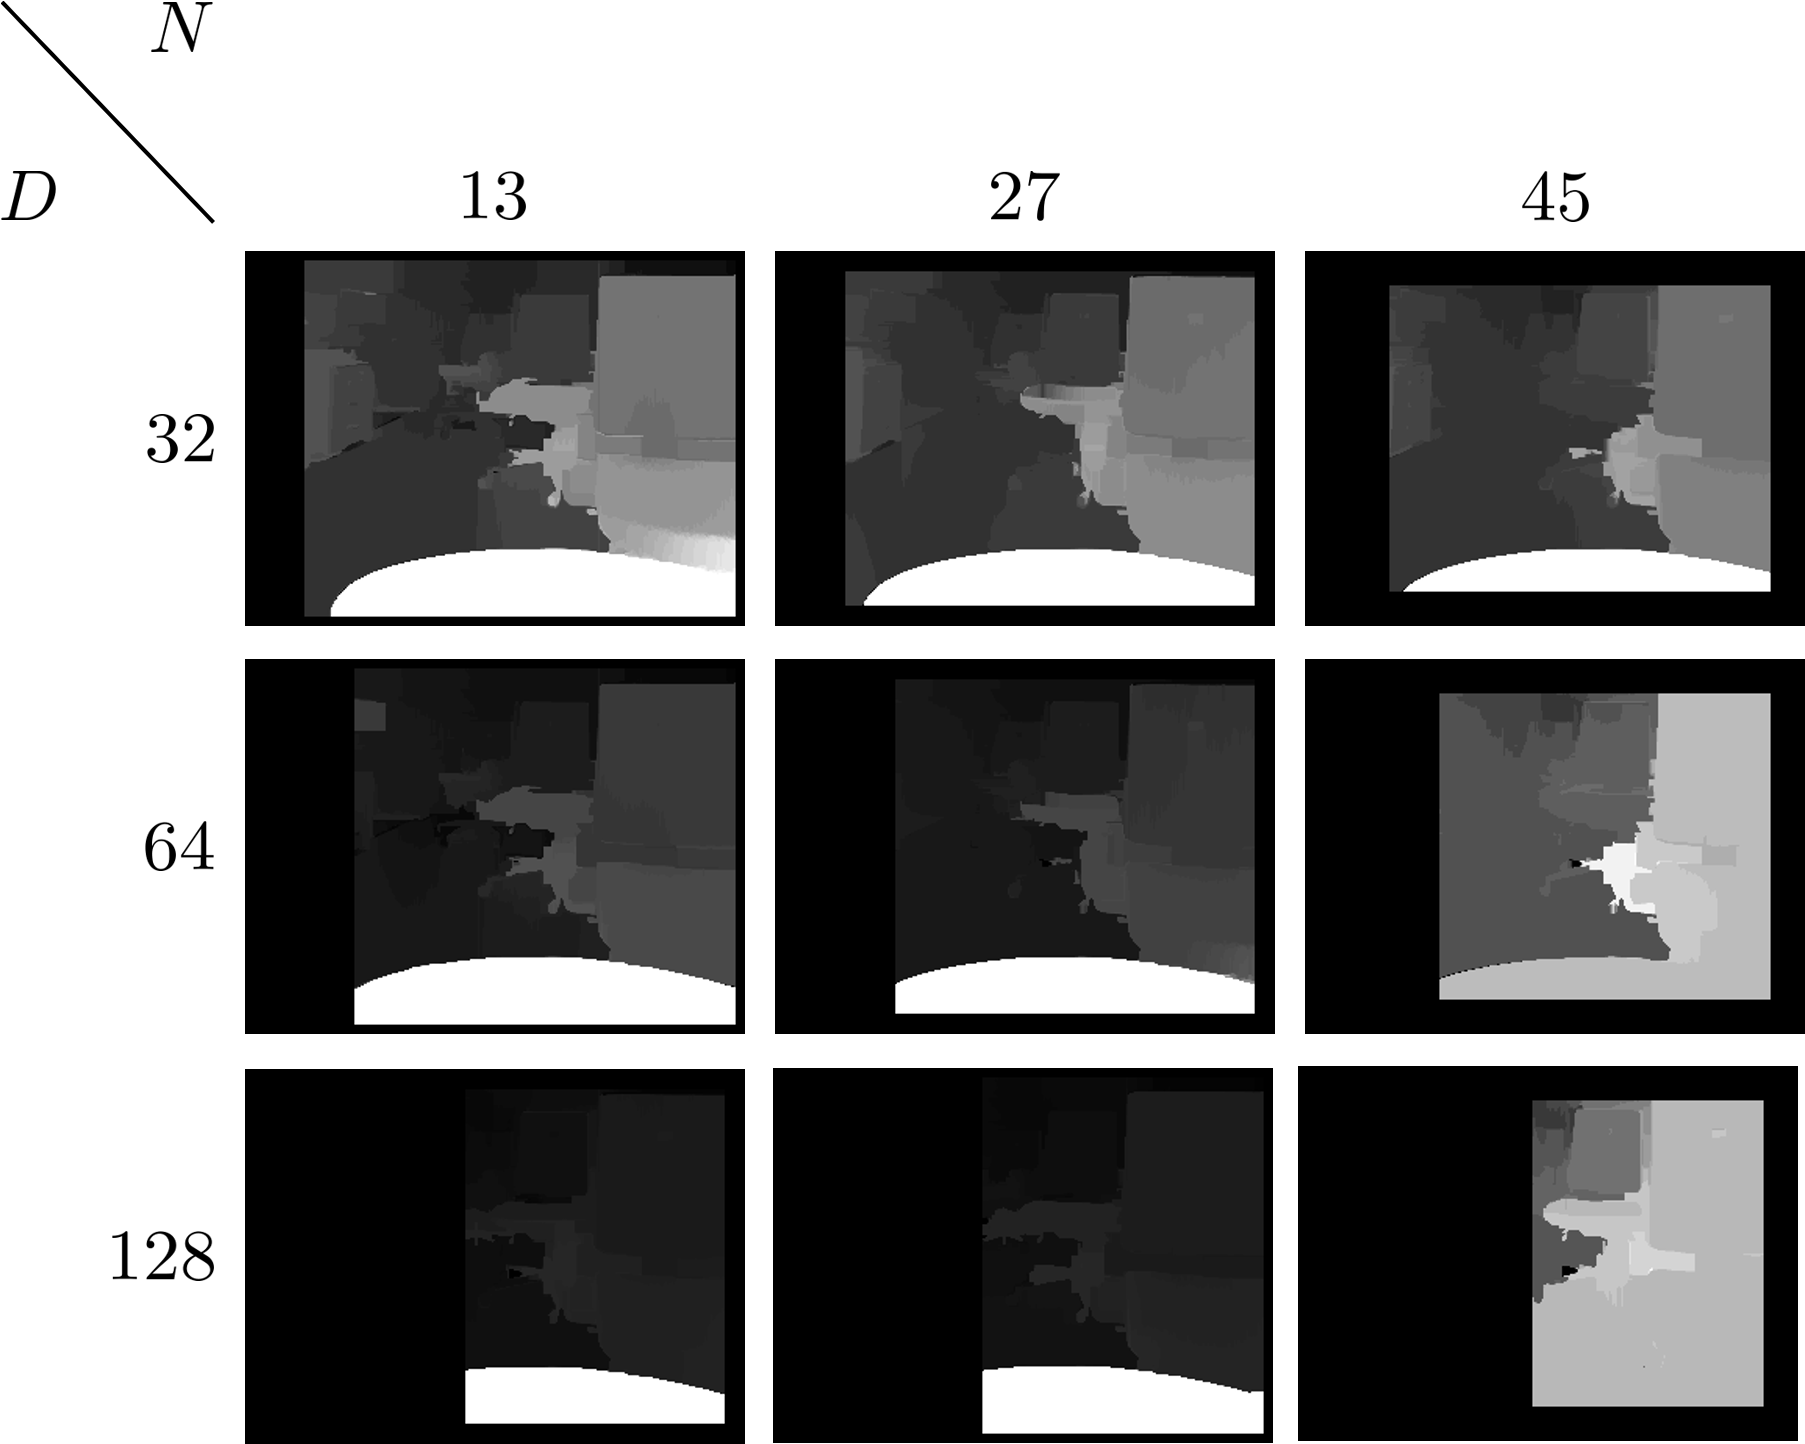
\includegraphics[scale=.25]{chapters/05_experiments/02_depth_map_parameter_tuning/disp_sad_wls.png}
	\caption{Confidence weighted least squares disparity for changing SAD windows sizes and number of disparities. Please refer to figure \ref{fig::324_weighted_least_squares_disparity} and equation \ref{eq::324_wls_final} for the theory.}
	\label{fig::52_disp_sad_wls}
\end{figure}
Within these depth maps, the global energy weighting $\lambda$ was set to $10^4$, and the local bilateral filter decay $\sigma$ to $1$, since we observed the best performance for them. The influence of those two parameters is visualized in figure \ref{fig::52_sigma_lambda}. We can see that, in good accordance with the theory, $\sigma$ contributes to the smoothing of the depth map, and that $\lambda$ enforces a change in depth across edges within the RGB images.
\begin{figure}[h]
	\centering
	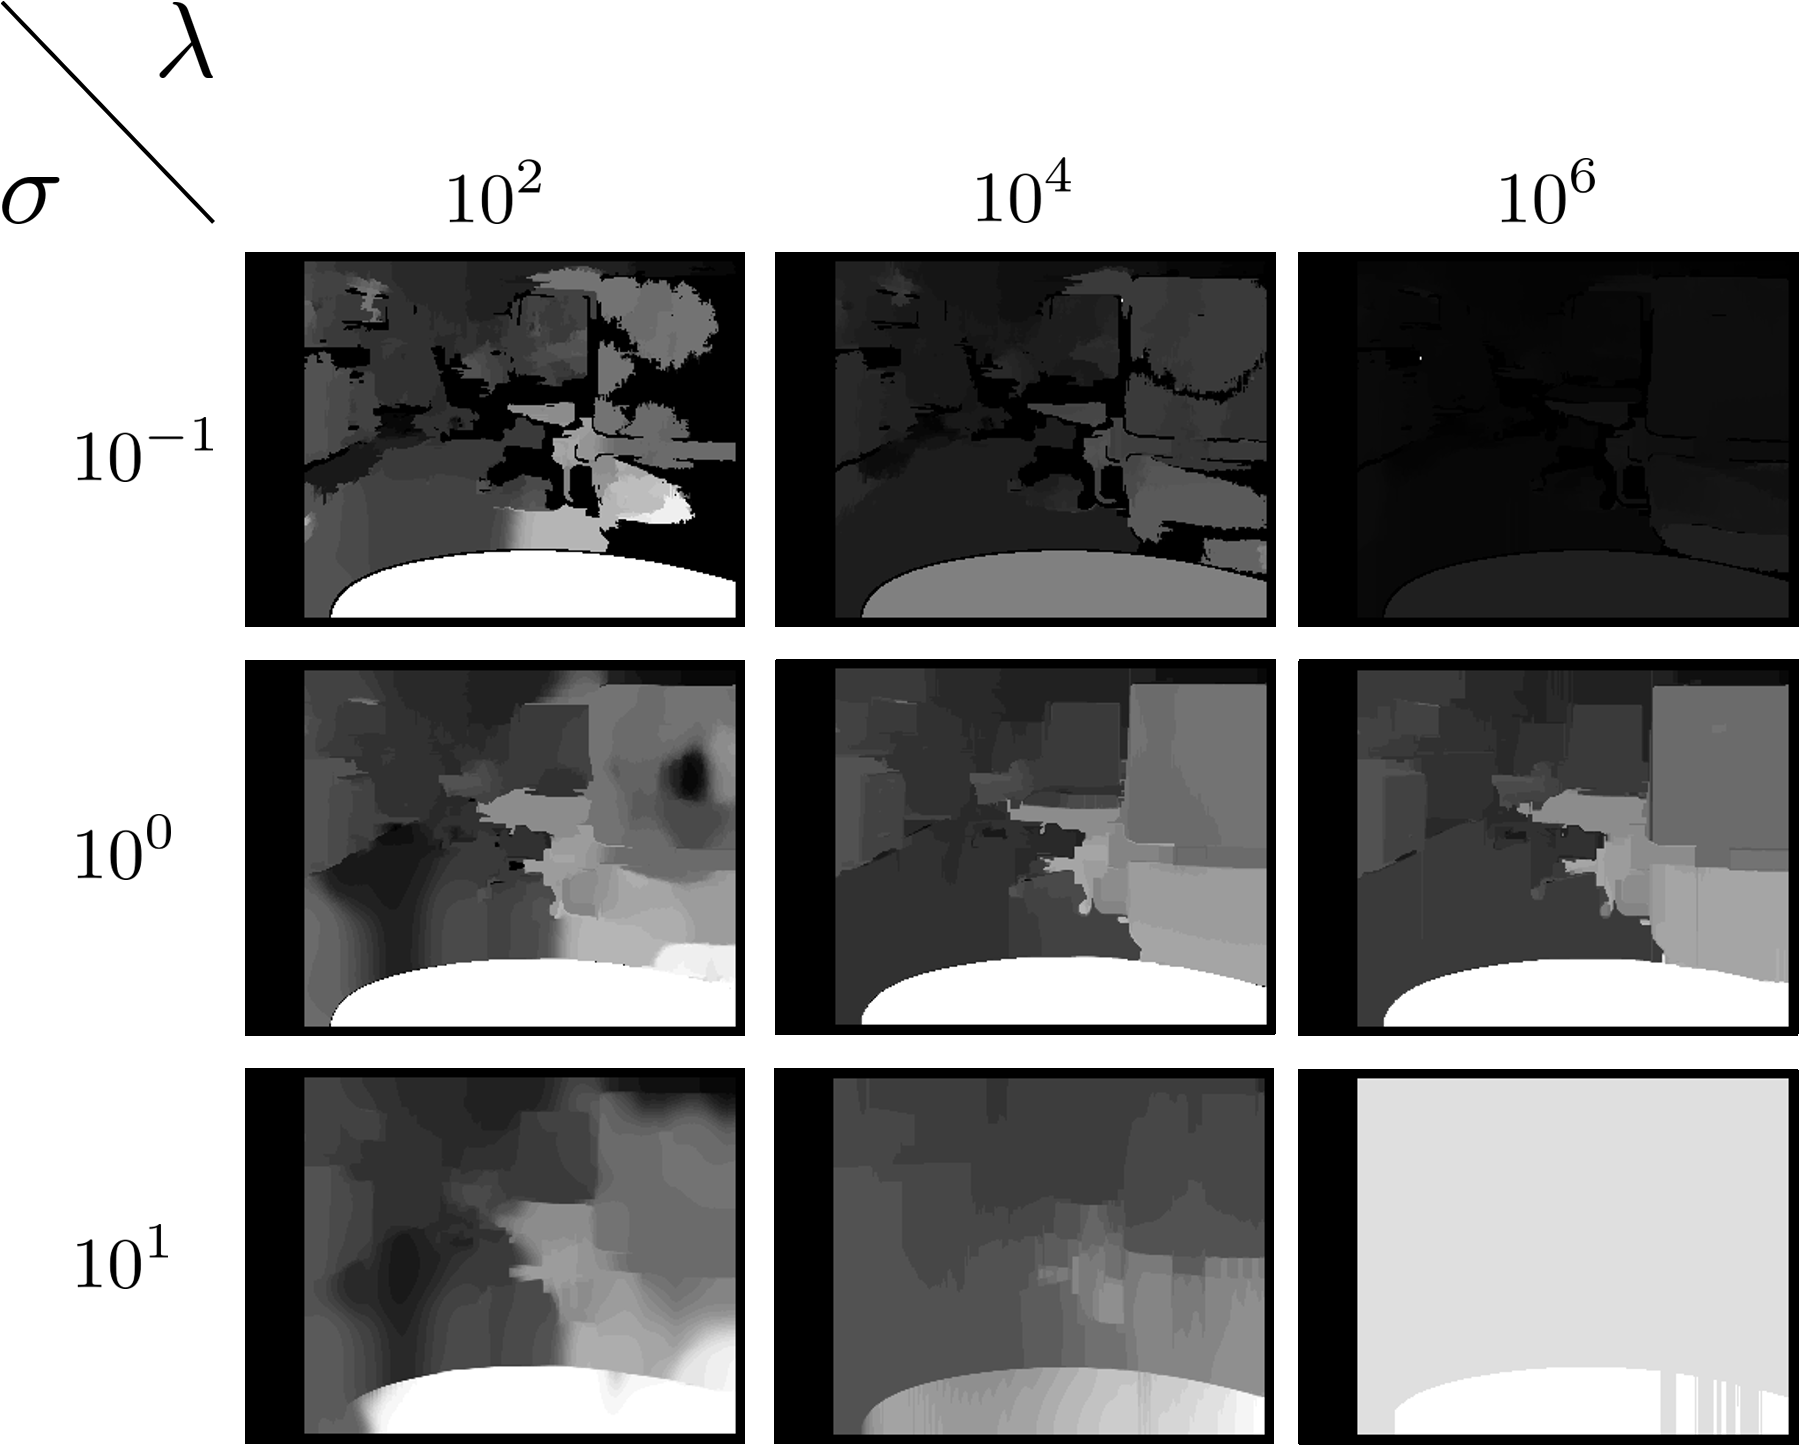
\includegraphics[scale=.25]{chapters/05_experiments/02_depth_map_parameter_tuning/sigma_lambda.png}
	\caption{Confidence weighted least squares disparity for changing energy weightings $\sigma$ and $\lambda$. Please refer to equations \ref{eq::324_weight} and \ref{eq::324_energy_function} for the theory.}
	\label{fig::52_sigma_lambda}
\end{figure}
For comparative purposes, we further demonstrate the depth map extraction without calibration in figure \ref{fig::52_no_calib}. 
\begin{figure}[h]
	\centering
	\subcaptionbox{Left disparity map.}%
	[.4\linewidth]{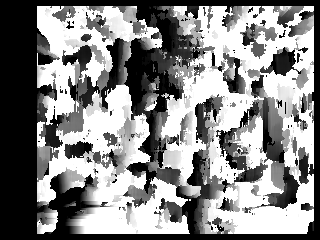
\includegraphics[scale=.3]{chapters/05_experiments/02_depth_map_parameter_tuning/disp_no_calib.png}}
	\subcaptionbox{Confidence weighted least squares filtered disparity map.}%
	[.4\linewidth]{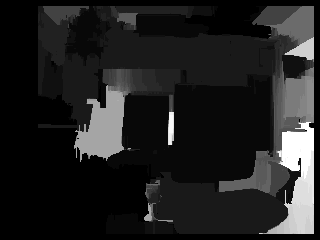
\includegraphics[scale=.3]{chapters/05_experiments/02_depth_map_parameter_tuning/wls_no_calib.png}}
	\caption{Depth map extraction without calibration. The parameters were set as follows to $N=13$, $D=32$, $\sigma = 1$, and $\lambda=10^4$.}
	\label{fig::52_no_calib}
\end{figure}